\chapter{Laplace transform}
Up until this point, the project has focused on the behaviour of electrical circuits in the time domain. Observing how different signals change with time yielded a differential equation, as seen in section (\ref{sec371}).
\\ \\
The solution to a differential equation will often be difficult to derive, and this is where the Laplace transform comes in handy. The Laplace transform converts functions of time to functions of frequency (i.e. from the time domain to the \textit{s}-domain). This process reduces the differential equation in question to an algebraic equation. Once the expression has been solved in the \textit{s}-domain, the inverse Laplace transform can be applied to find its corresponding solution in the time domain. Generally, this description can be illustrated in the following way:
\begin{figure}[H]
 \center
 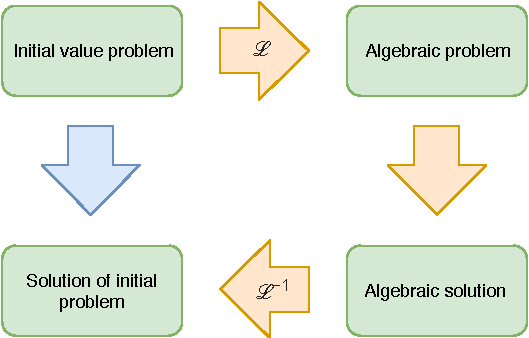
\includegraphics[scale=1]{fig/img/laplace_circ.pdf}
 \caption{Solution using Laplace}
\end{figure}

\section{The Laplace Transform}
\begin{tcolorbox}[colback=blue!5!white,colframe=blue!75!black,title=Definition]
\begin{align}
\mathcal{L}\{f(t)\}=F(s)=\int_{0}^{\infty} e^{-st}\cdot f(t)\ dt
\label{lpdef}
\end{align}
where $f(t)$ is a function of time, $F(s)$ is the Laplace transform of that very function, and $s$ is a complex variable.
\end{tcolorbox}

\begin{tcolorbox}[colback=red!5!white,colframe=red!55!black,title=Example of a Laplace transform]
In (\ref{lpdef}), let $f(t)=e^{at}$, where $a$ is a constant, and $t$ is time. In that case,
$$\mathcal{L}\{f(t)\}=\int_{0}^{\infty} e^{-st}\cdot e^{at}\ dt$$
Since they have the base, $e$, in common, their exponents can be combined. Additionally, $t$ can be factorised:
$$\mathcal{L}\{f(t)\}=\int_{0}^{\infty} e^{-(s-a)t}\ dt$$
If $u=-(s-a)t$, then integration by substitution yields $dt=-\dfrac{1}{(s-a)}\ du$. Thus:
\begin{align}
\mathcal{L}\{f(t)\}=\int_{0}^{\infty} e^{u}\cdot (-\dfrac{1}{(s-a)})\ du =  -\dfrac{1}{s-a} \cdot \left[e^{-(s-a)t} \right]_{0}^{\infty}
\label{eq6.2}
\end{align}
Applying the limits of integration to (\ref{eq6.2}), and letting N approach $\infty$. Furthermore, the The equation is going to look as follows:
\begin{align*}
\mathcal{L}\{f(t)\} = \lim_{N \to \infty} -\dfrac{1}{s-a} \cdot \left[e^{-(s-a)t} \right]_{0}^{N} =-\dfrac{1}{s-a}\cdot (e^{-(s-a)N}-e^{0})=\dfrac{1}{s-a}
\end{align*}
In conclusion, the Laplace transform of $f(t)=e^{at}$ equals
$$\mathcal{L}\{f(t)\}=\dfrac{1}{s-a} \ \ \ ;\ \ \ s>a$$
$s$ must be greater than $a$, since the limit of $e^{-(s-a)N}$ converges towards zero. If $a$ is greater than $s$, the exponent of $e$ would be positive, and the limit would diverge. 
\end{tcolorbox}
The Laplace transform can be used for all functions of $f$, where the real part of $s$ is greater than $a$ $Re(s)>=a$. Since $s$ is a complex number ($s=a+ib$), only the first part of $s$ has to be greater than $a$. Therefore, $e^{-st}$ is  the same as $e^{-ta}e^{-tib}$, where the last part is the imaginary part of the complex number. In the complex chapter, this is also defined as $e^{a}\cos(b)+ i \sin(b)$. Since the imaginary parts are defined as functions of cosine and sinus, they can not approach $\infty$. Therefore, only the real part of $s$ from equation \eqref{lpdef} can approach $\infty$, and is only going to converge when $Re(s) >= a$, and diverge when $Re(s)<a$.
\\ \\
The Laplace transform can be applied to the derivatives of multiple orders. In particular, the Laplace transform of the first order derivative, since it is essential when looking at the high and low-pass filters. 
%mere tekst/bedre overgang
\begin{tcolorbox}[colback=green!5!white,colframe=green!40!black,title=Theorem 6.1: Laplace transform of a first order derivative]
The Laplace-transform of a first order derivative takes the following form:
$$\mathcal{L}\{\frac{df}{dt}\} = s\cdot F(s)-f(0)$$
\end{tcolorbox}

\begin{tcolorbox}[colback=gray!5!white,colframe=gray!!black,title=Proof 6.1]
Integration by parts states that 
\begin{align}
\int_{a}^{b}{u\cdot v}=\left[u\cdot v\right]_{a}^{b}-\int_{a}^{b} \frac{du}{dt}\cdot v\
\label{eq6.3}
\end{align}

In this case, $u=e^{-st}$ and $v=f(t)$.
Equation (\ref{eq6.3}) then yields
$$\mathcal{L}\{\frac{df}{dt}\}=\left[e^{-st}\cdot f(t)\right]_{0}^{\infty}-\int_{0}^{\infty} -s\cdot e^{-st}\cdot f(t)\ dt$$

To rewrite, use that $\frac{1}{a}=a^{-n}$. Additionally, since $s$ is merely a constant, it can be placed in front of the integral. When applying the limits of integration to the first term, let $N$ approach infinity, such that
\begin{align}
\mathcal{L}\{\frac{df}{dt}\}=\lim_{N \to \infty}\left[\dfrac{1}{e^{st}}\cdot f(t)\right]_{0}^{N}+s\cdot \int_{0}^{\infty}e^{-st}\cdot f(t)\ dt
\label{eq6.4}
\end{align}

Note, that the second term of (\ref{eq6.4}) now equals the product of $s$ and $\mathcal{L}\{f(t)\}$. 
$$\mathcal{L}\{\frac{df}{dt}\} = \lim_{N \to \infty}\left[\dfrac{1}{e^{s\cdot N}}\cdot f(N)-\dfrac{1}{e^{s\cdot 0}}\cdot f(0)\right]+s\cdot \mathcal{L}\{f(t)\}$$

Since $$\lim_{N \to \infty}\left[\dfrac{1}{e^{s\cdot N}}\right]=0$$ then, naturally, any other number multiplied by 0 will also equal to 0.\\
In conclusion, this results to
\begin{align*}
\mathcal{L}\{\frac{df}{dt}\} = s\cdot \mathcal{L}\{f(t)\}-f(0)
\end{align*}
\end{tcolorbox}